
\section{Tratamiento de datos} % (fold)
\label{sec:tratamiento_de_datos}

\begin{table}[!htbp]
\centering
\resizebox{\textwidth}{!}{

\begin{tabular}{lllllllrr}
\toprule
               Dates &        Category &     Descript &  DayOfWeek & PdDistrict &      Resolution &                  Address &           X &          Y \\
\midrule
 2008-04-15 18:30:00 &   DRUG/NARCOTIC &  POSSESSI... &    Tuesday &       PARK &  JUVENILE CITED &  700 Block of STANYAN ST & -122.453513 &  37.768697 \\
 2011-08-25 18:33:00 &        WARRANTS &  WARRANT ... &   Thursday &   SOUTHERN &  ARREST, BOOKED &   900 Block of MARKET ST & -122.408421 &  37.783570 \\
 2007-09-09 02:32:00 &     DRUNKENNESS &  UNDER IN... &     Sunday &   SOUTHERN &  ARREST, BOOKED &  1400 Block of FOLSOM ST & -122.413772 &  37.772142 \\
 2012-09-08 23:59:00 &   LARCENY/THEFT &  GRAND TH... &   Saturday &  INGLESIDE &            NONE &   100 Block of EMMETT CT & -122.416079 &  37.747295 \\
 2004-03-17 16:00:00 &   LARCENY/THEFT &  GRAND TH... &  Wednesday &   SOUTHERN &            NONE &   CLEMENTINA ST / 5TH ST & -122.403924 &  37.780699 \\
 2014-06-01 00:20:00 &        BURGLARY &  BURGLARY... &     Sunday &   NORTHERN &            NONE &  1300 Block of SUTTER ST & -122.422586 &  37.787387 \\
 2008-07-10 18:15:00 &  OTHER OFFENSES &  DRIVERS ... &   Thursday &   SOUTHERN &   ARREST, CITED &     HARRISON ST / 1ST ST & -122.392941 &  37.786068 \\
 2003-05-13 12:00:00 &   LARCENY/THEFT &  PETTY TH... &    Tuesday &   NORTHERN &            NONE &  0 Block of CERVANTES BL & -122.438303 &  37.803634 \\
 2013-04-07 19:00:00 &    NON-CRIMINAL &  FOUND PR... &     Sunday &   SOUTHERN &            NONE &     300 Block of 10TH ST & -122.412410 &  37.772404 \\
 2014-06-25 22:15:00 &   LARCENY/THEFT &  GRAND TH... &  Wednesday &   SOUTHERN &            NONE &      FOLSOM ST / 10TH ST & -122.412827 &  37.772812 \\
\bottomrule
\end{tabular}


}
\caption{Algunos datos aleatorios del set de entrenamiento}
\end{table}

\subsection{Explorando el set de datos} % (fold)
\label{sub:explorando_el_set_de_datos}

Los sets de datos son extensos. Para darnos una idea de como están compuestos podemos tomar una muestra, y analizarla. Cada fila del set representa un crimen. Las filas vienen con una fecha completa, el distrito donde pasó el crimen, el día de semana, la dirección, la latitud y la longitud exactas. El set de entrenamiento también viene con el tipo de cada crimen (los que justamente necesitamos deducir sobre el set de prueba), y con una descripción y resolución de cada crimen. Estos últimos dos no nos interesan, ya que no aparecen en el set de prueba y, por ende, no podremos tomar ninguna decisión en base a ellos.

Pero para entender mejor el set de datos, lo graficaremos. Teniendo, por ejemplo, el gráfico de categorías~\ref{fig:categories} ya podemos hacer deducciones sobre nuestro set de entrenamiento. Es muy visible que los crímenes no están uniformemente distribuidos, por ende lo más probable es que en la deducción casi siempre vamos a tender a darle más probabilidad a \textit{LARENCY/THEFT} o \textit{OTHER OFFENSES}.

\begin{figure}[H]
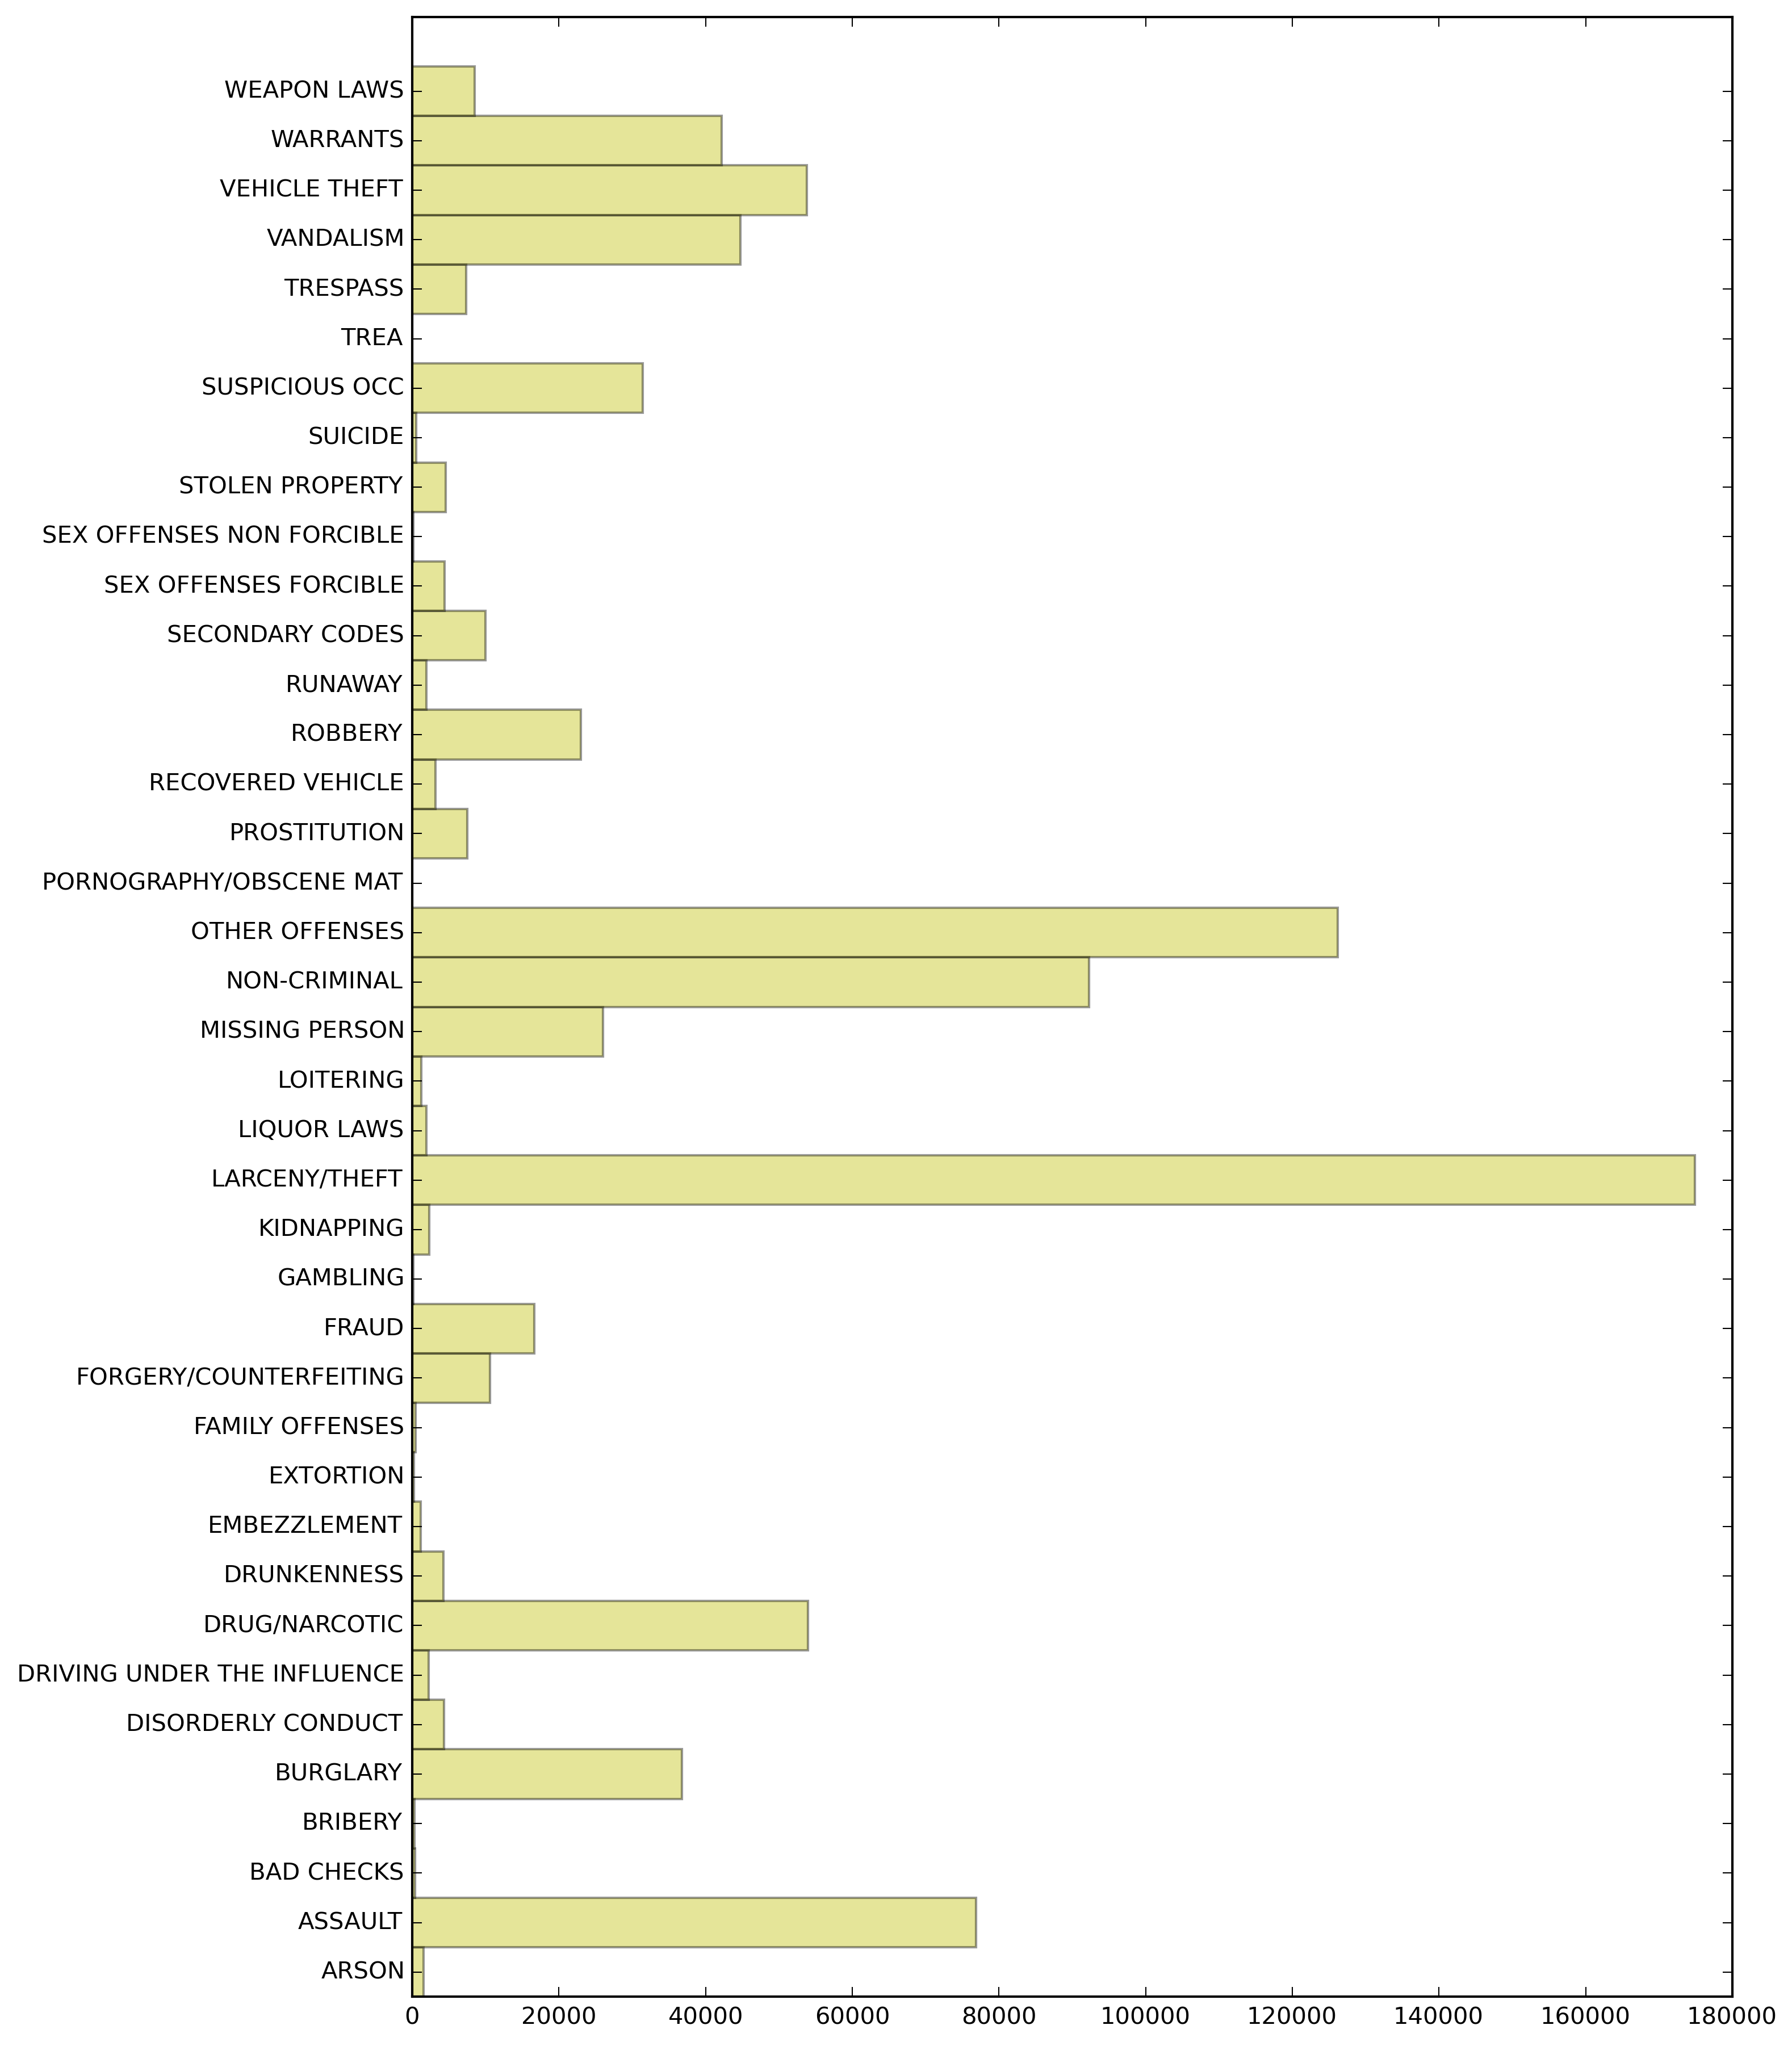
\includegraphics[width=130mm]{categories}
\caption{Cantidad de crímenes de cada tipo.}
\label{fig:categories}
\end{figure}

% subsection explorando_el_set_de_datos (end)

\subsection{Deduciendo features} % (fold)
\label{sub:deduciendo_features}

Como parte de preprocesamiento, necesitaremos deducir cuáles son los datos importantes para nosotros, es decir cuáles son los datos que van a ayudar a que nuestro algoritmo aprenda más eficientemente y prediga mejor. Esos datos se pueden encontrar directamente en el set de datos tal como está o pueden necesitar algún procesamiento previo. Algunos inclusive pueden ser combinación de varios datos de una fila.

Los únicos datos discretos, que sirven directamente son el distrito y el día de semana. La fecha tal como viene no tiene valor: cada crimen tiene una fecha única y lo más probable es que en el set de prueba tampoco se repita. Necesitamos procesar esa fecha primero.

\begin{figure}[H]
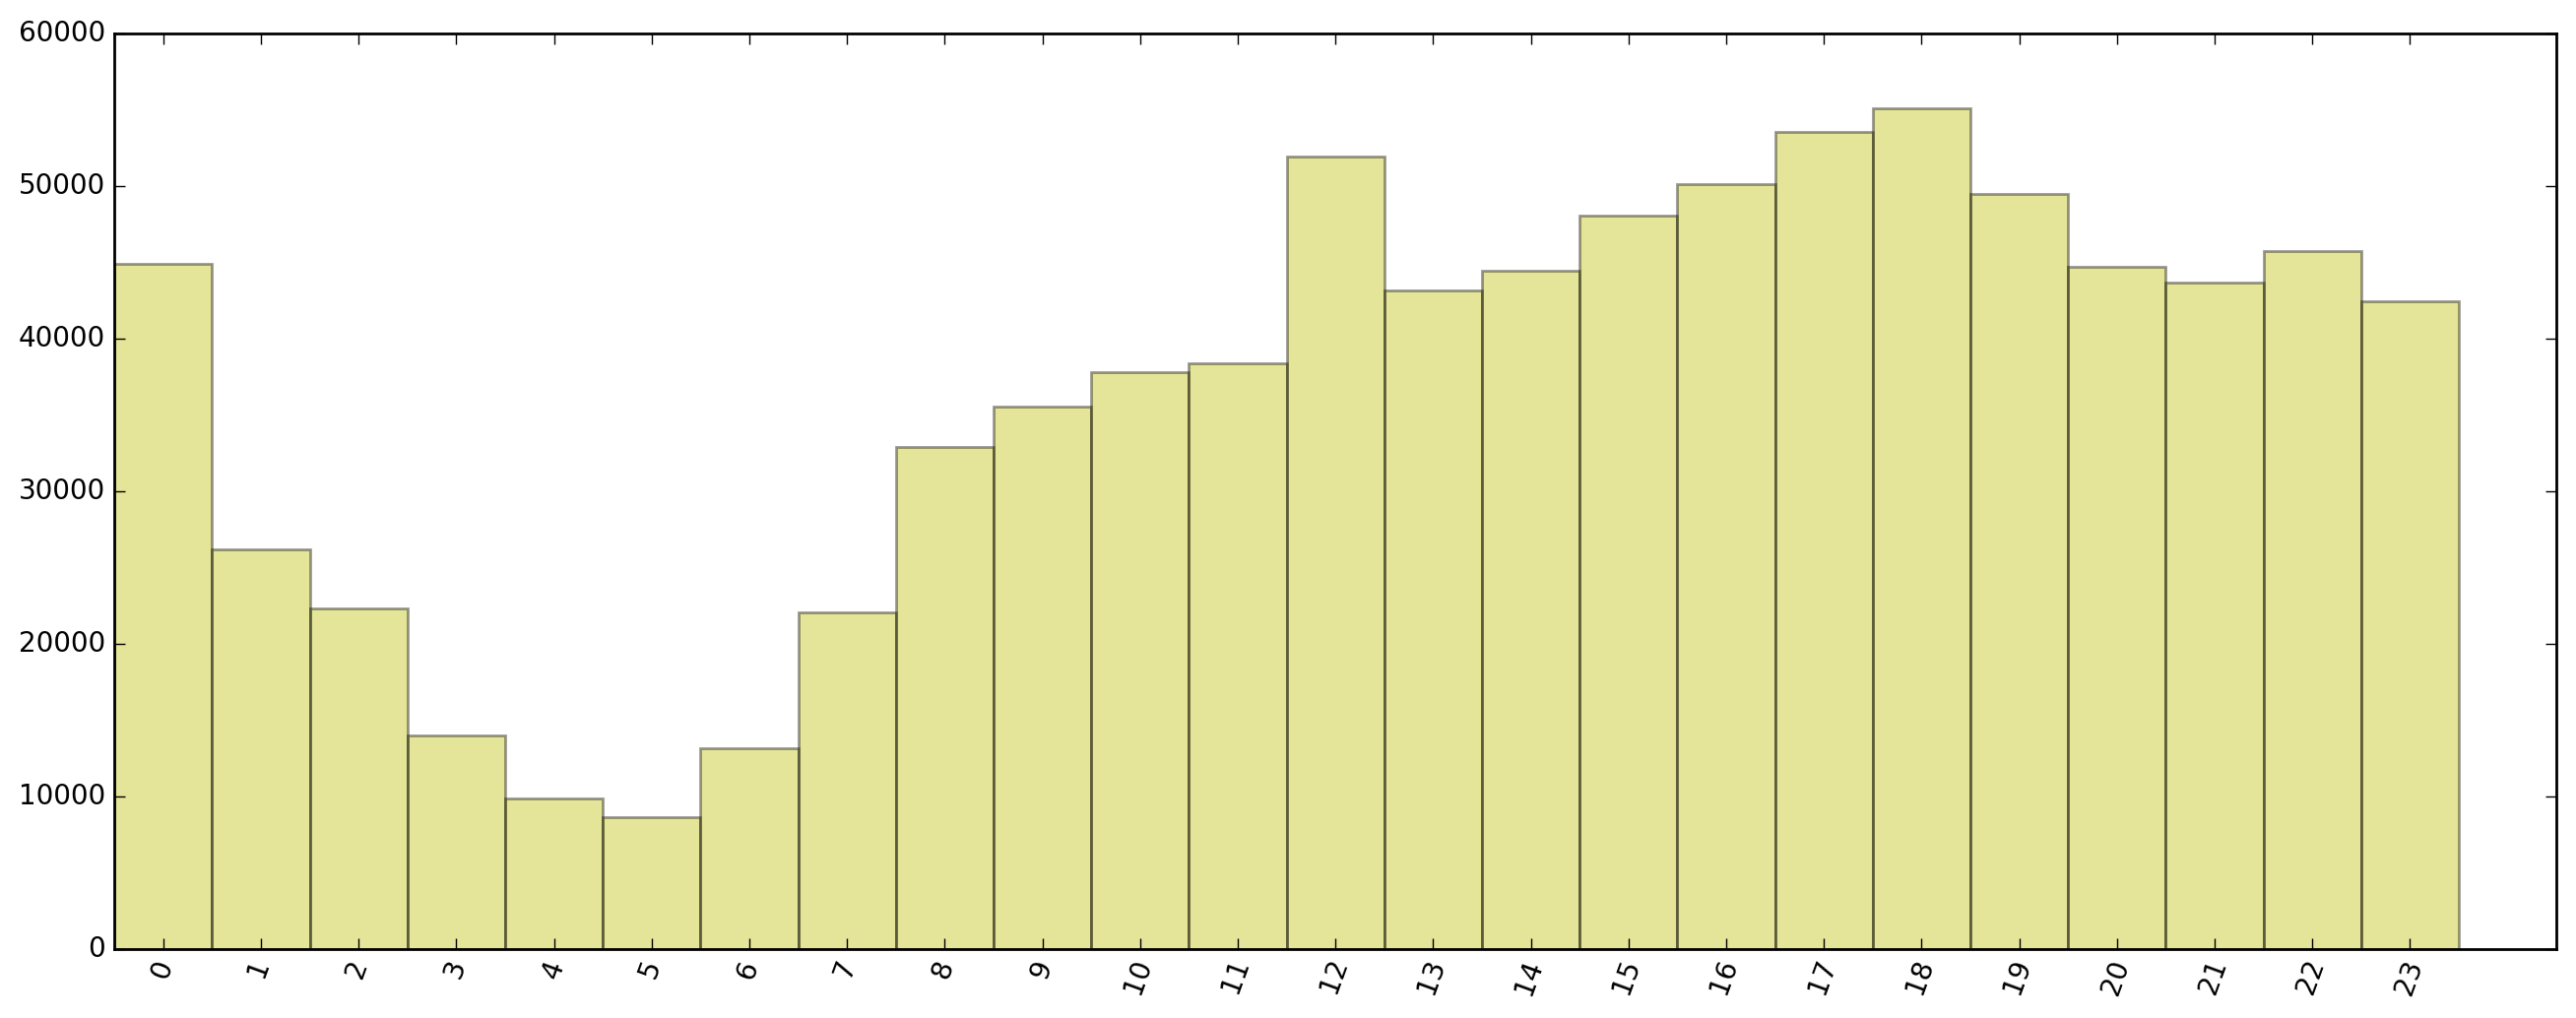
\includegraphics[width=160mm]{hours}
\caption{Cantidad de crímenes por hora.}
\label{fig:hours}
\end{figure}

Fecha es un dato muy útil, algunos features resultantes del procesamiento de ella que vienen inmediatamente a la mente son: la hora, el mes, el año. Pero podemos sacar otros features no menores, por ejemplo deducir si era verano o invierno, si era de día o de noche (inclusive variar el rango de día y de noche según estación, siendo que en invierno oscurece más temprano). Sí observamos el gráfico~\ref{fig:hours}, podemos detectar que entre la una y las siete la cantidad de crímenes baja notablemente y, por lo contrario, hay dos picos a las 12 y a las 18. Todos esos datos se pueden convertir en features para nuestro algoritmo. También podemos sacar el dato sobre el día de semana de la fecha - de esta forma la columna con el día de semana en los sets es, en realidad, redundante. Si podemos conseguir datos externos, podríamos que fechas fueron feriado.

La dirección a priori no es un dato tan fuerte como la fecha, y también necesita procesamiento. Podríamos sacar nombres de calles o abusarnos de la notación y deducir que crímenes ocurrieron en las esquinas (las dirección de las esquinas están denotadas como ``Calle 1 / Calle 2''.

La longitud y la latitud es a simple vista un dato muy importante y a la vez difícil de procesar. Eso pasa por el hecho de que por separado claramente no tienen sentido. Vamos a tener que encontrar una forma de convertirlos en algo útil para nuestros algoritmos. Una manera podría ser encontrar alguna función que devuelva un número muy parecido para X e Y cercanos. Otra sería dividir las longitudes y latitudes en zonas, y ver en que zona se encuentra la fila. Este enfoque puede conducir a errores ya que para ser preciso va a necesitar más zonas. Algo útil podría resultar una búsqueda de datos externos con latitudes y longitudes de lugares particulares de San Francisco, como pueden ser las estaciones de policía (distancia a ellos podría ser un feature interesante), o determinar si el crimen pasó en un parque.

\begin{figure}[H]
\centering
\begin{subfigure}{.5\textwidth}
  \centering
  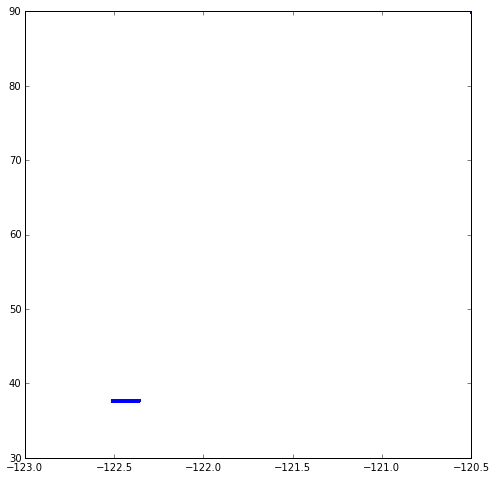
\includegraphics[width=.8\linewidth]{xy1}
  \caption{Set de entrenamiento}
  \label{fig:xy1}
\end{subfigure}%
\begin{subfigure}{.5\textwidth}
  \centering
  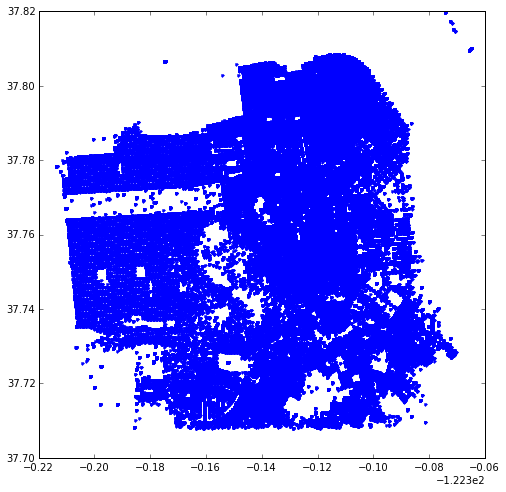
\includegraphics[width=.8\linewidth]{xy2}
  \caption{Sin datos incorrectos}
  \label{fig:xy2}
\end{subfigure}
\caption{Gráficos de latitudes y longitudes de los crímenes}
\label{fig:xy}
\end{figure}

Si graficamos la latitud en función de la longitud, lo primero que vamos a obtener es algo parecido al gráfico de~\ref{fig:xy2}: nos encontramos con que algunas de las filas tienen datos incorrectos. Hay 67 crímenes con latitudes y longitudes incorrectas. Si bien podríamos descartarlos - su impacto es minucioso frente al set entero, pero es posible, por ejemplo determinar su X e Y correcto a partir de los crímenes que pasaron en las mismas direcciones. Y para los que queden sin clasificar - podríamos ubicarlos en lugares aleatorios de San Francisco.

% subsection deduciendo_features (end)


\subsection{Transformando datos} % (fold)
\label{sub:transformando_datos}

El set de datos proporcionado en su estado inicial no sirve para aplicarle los algoritmos típicos de machine learning: un algoritmo matemático no tiene una forma práctica de interpretar los datos que contiene. Los datos que mejor puede interpretar son números. Entonces está entre nuestras necesidades el convertir los sets de datos heterogéneos en matrices numéricas.

Todos los features necesitan ser escalados a un rango de números (puede ser entre 0 y 1, o entre -1 y 1). De esta manera el algoritmo tiene menor chance de equivocarse dándole mayor peso a features con mayor valor numérico (como puede ser el año con respecto al mes).

¿Pero como hacemos para representar numéricamente si un crimen pertenece a un distrito? Una de las solución es utilizar codificación \textit{one-hot} (o variables \textit{dummy}). Este método consiste en, en vez de representar alguna variable categórica, como puede ser el distrito, con un solo feature, representarlo con un feature por cada categoría existente, marcando si es o no es de esa categoría (con un 1 o un 0). De esa manera a partir de la columna de Distrito tendríamos 10 features diferentes, donde cada fila tendría un 1 en uno de ellos - y 0 en el resto. Lo mismo es posible hacerlo con los días de semana, meses, años, zonas de latitudes y longitudes, y hasta calles - pero es necesario hacer un análisis previo y decidir si tiene sentido o no.

% subsection transformando_datos (end)

% section tratamiento_de_datos (end)
